\documentclass[journal]{IEEEtran}
\usepackage[utf8]{inputenc}
\usepackage[T1]{fontenc}
\usepackage{amsmath,amssymb,amsfonts}
\usepackage{graphicx}
\usepackage{booktabs}
\usepackage{adjustbox}
\usepackage{cite}
\usepackage{url}
\usepackage{textcomp}
\usepackage{newunicodechar}
\newunicodechar{µ}{\ensuremath{\mu}}
\newunicodechar{±}{\ensuremath{\pm}}
\newunicodechar{×}{\ensuremath{\times}}
\newunicodechar{−}{\ensuremath{-}}
\newunicodechar{≥}{\ensuremath{\geq}}
\newunicodechar{≤}{\ensuremath{\leq}}
\newunicodechar{Φ}{\ensuremath{\Phi}}
\newunicodechar{γ}{\ensuremath{\gamma}}
\newunicodechar{ρ}{\ensuremath{\rho}}
\newunicodechar{λ}{\ensuremath{\lambda}}
\newunicodechar{Δ}{\ensuremath{\Delta}}
\newunicodechar{ℓ}{\ensuremath{\ell}}
\newunicodechar{→}{\ensuremath{\rightarrow}}
\newunicodechar{​}{}
\providecommand{\tightlist}{\setlength{\itemsep}{0pt}\setlength{\parskip}{0pt}}
\def\UrlBreaks{\do\/\do-\do.}
\hyphenation{EPARA TRACE}
\begin{document}
\title{TRACE: Trust-Constrained, Category-Aware Request Routing for AI Inference in Edge-Cloud Collaborative Systems}
\author{Nithish~Kumar, Ganesh~Khekare$^{*}$, and Gaurav~Nitesh~Gandhi\\[4pt]
{\normalsize School of Computer Science and Engineering, Vellore Institute of Technology, Vellore, Tamil Nadu, India}\\
{\normalsize nithishkumar.r2023@vitstudent.ac.in, ganesh.khekare@vit.ac.in$^{*}$, gauravnitehs.gandhi2023@vitstudent.ac.in}\\
{\normalsize $^{*}$Corresponding author}}
\maketitle

\begin{abstract}
Edge-cloud collaborative systems increasingly serve AI inference on fragmented, heterogeneous edge servers. Decentralized request handlers such as EPARA's offload requests to peers in proportion to their idle capacity, but treat every server that hosts a model as a lawful destination. We formulate trust-constrained routing as goodput maximization subject to zero violations, using multilevel-security labels (clearance and trust domain), an explicit threat model in which ingress servers relay but do not process data, and a closed-form expression showing that the violation rate of trust-oblivious routing is fixed by the label distributions. We present TRACE, a decentralized router that combines a hard trust filter, SLO-aware admission and an adaptively enabled best-fit clearance preference with capacity-proportional offloading, at about 20 µs per decision. In simulation with 30 heterogeneous servers, 30 evaluation seeds and Holm-corrected paired tests, compliance costs 1.2 points of SLO attainment for a centralized dispatcher with perfect information and 2.7 points for decentralized routing at the default traffic mix, rising with the share of sensitive traffic. TRACE attains 0.960 compliant SLO attainment at 80\% load, 2.9 points below the centralized oracle; it is tied with a trust-filtered join-the-shortest-queue router below saturation and ahead of it, of trust-filtered power-of-two-choices and round-robin routing and of static per-tier pools at and beyond saturation (by 8 to 34 points at 100\% load). SLO-aware admission is the decisive element in overload, raising every router's attainment at 100\% load by more than 50 points. Aligning data sensitivity with ingress clearance reduces, but does not remove, violations of trust-oblivious offloading (13.5\% at full alignment). We also test whether weighting offload decisions by energy headroom helps on energy-constrained sites: it is harmful when energy is scarce and an empty buffer throttles work (9.2 points), gives small gains that are not significant after correction under hard outages, and is neutral when supply is sufficient. All parameters are documented assumptions, and the simulator and raw results are public.
\end{abstract}

\begin{IEEEkeywords}
Edge-cloud collaborative computing, AI inference serving, request offloading, multilevel security, trust domains, admission control, energy-aware scheduling
\end{IEEEkeywords}

\section{Introduction}

Workloads based on inferencing are moving towards the ``edge'' in networks. Video analytics applications, voice assistant applications and robotic control applications require their responses to be delivered within tens to hundreds of milliseconds, and all of these applications take input from consumers who are subject to increasing amounts of privacy regulation. The response has been an architecture known as ``edge-cloud collaborative computing,'' which uses a three-tiered architecture: the first tier consists of edge servers that are located near the consumer and perform nearly all of the workload; when edge servers cannot handle additional workload, the workload is passed to other edge servers or to the cloud \cite{liu2025eccc}. Each individual edge server is relatively small and the set of edge servers is heterogeneous; however, there exists a significant amount of combined idle capability across the entire set of servers if incoming requests can be routed quickly to available servers.

EPARA \cite{epara2025} is a recent example of this type of architecture. EPARA classifies inference services along two dimensions: whether a service is latency-sensitive or frequency-sensitive, and whether it needs less or more than one graphics processing unit (GPU). Based upon this classification, EPARA selects a parallelization strategy for each class. A decentralized request handler is used to determine when to keep a request at its current location and when to forward the request to a peer edge server. When deciding where to send a request, the request handler uses a probabilistic decision rule where the probability of sending the request to a given peer is directly related to that peer's idle goodput. At a regular interval, EPARA also uses a placement mechanism to move models closer to demand. EPARA was evaluated through comparison to several previously developed architectures for serving both edge and centralized inference services \cite{epara2025}.

All of the previous architectures \cite{interedge,galaxy,servp,alpaserve,usher} were designed so that any server that hosts a model can receive any request. In real-world scenarios this assumption often does not hold. For example, imaging data collected by a hospital may need to be processed only by certified operators. Similarly, residency restrictions may confine data processing within an organizational or governmental boundary \cite{gdpr,hummel2021}. A router that does not enforce these types of constraints can indicate high levels of goodput even though some portion of the traffic being served could be considered unlawful. A second implicit assumption concerns energy: many edge sites are power-capped, solar-powered or battery-backed, and steering work toward servers with spare energy, as energy-aware offloading does for mobile devices \cite{mao2016harvest}, looks like an obvious refinement.

As such, we address request routing as a constrained optimization problem: maximize timely service while ensuring all requests are processed within their respective trust boundaries. Two questions then emerge. How much timely service does a fast decentralized router lose by complying with the trust constraints, measured against unconstrained and centralized references, and which routing rules minimize this loss? Additionally, does energy awareness in making offload decisions help, and at what levels of available supply?

The authors' contributions include:

\begin{itemize}
\item
  \textbf{Model.} The authors provide a model for trust-constrained routing of categorized edge inference. This includes multi-level security labels (clearance and trust domain) and the stated threat model; the threat model describes how ingress servers forward data even if they are not permitted to process it. Additionally, a closed-form expression is provided for the violation rate of trust-oblivious routing, demonstrating that the violation rate is determined by the distribution of the labels, and not by the behavior of the router itself (Section III).
\item
  \textbf{Design.} The authors extend capacity-proportional offloading with a hard trust filter and a best-fit clearance preference, which each server switches on once it has observed sufficient sensitive traffic. Furthermore, SLO-aware (Service Level Objective) admission is used to shed, or send to the cloud, those requests that can no longer meet their SLO deadlines. Each decision takes approximately tens of microseconds of local processing time (Section IV).
\item
  \textbf{Evaluation against strong references.} The authors evaluate TRACE against five reference routers: trust-filtered round-robin, power-of-two-choices and join-the-shortest-queue routing, static per-tier pools, and a centralized dispatcher that has perfect knowledge. The evaluation uses thirty evaluation seeds, and all comparisons use Holm-corrected paired tests. Additionally, the authors vary the correlation between data sensitivity and ingress clearance, the proportion of sensitive traffic, overload conditions, state staleness, placement, the availability of a cloud fallback, network topology and every routing parameter (Section VI).
\item
  \textbf{Energy-aware routing as a testable hypothesis.} Five energy-aware variants are described and evaluated, including a feasibility oracle that has perfect knowledge of energy, over supply ratios below and above demand, constant and phase-shifted solar supply, and short and long battery buffers; the mechanisms behind the results (load dispersion, availability and forwarding) are measured directly (Section VII).
\end{itemize}

All results come from simulation with documented, assumed parameters at the scale of EPARA's testbed. They are not hardware measurements and should not be compared in absolute terms with EPARA's reported numbers.

\section{Background and Related Work}

\textbf{Categorized parallel inference at the edge.} EPARA \cite{epara2025} categorizes inference tasks along two axes and applies five operators accordingly: batching, multi-task co-location, model parallelism, multi-frame batching and request-level data parallelism. It couples this allocator with a decentralized request handler that offloads a request to a peer with probability proportional to the peer's idle goodput, a submodular service-placement algorithm with a \(1/(1+P)\) guarantee \cite{fisher1978submodular}, and ring-based state synchronization. Its handler, like those of the edge systems it compares against (InterEdge \cite{interedge}, Galaxy \cite{galaxy}, SERV-P \cite{servp}) and of datacenter serving systems (AlpaServe \cite{alpaserve}, USHER \cite{usher}, Nexus \cite{nexus}, SHEPHERD \cite{shepherd}, Clockwork \cite{clockwork}, INFaaS \cite{infaas}), treats every server that hosts a model as a valid destination. We study EPARA's \emph{request-handling} layer. Its operators are not modelled mechanistically: we reduce each category to a fixed slot and service-time profile (Section V), so batching gains and co-location interference are outside the scope of this paper.

\textbf{Edge-cloud collaborative intelligence.} A recent survey \cite{liu2025eccc} organizes ECCC research into model optimization, AI-driven resource management and privacy/security enhancement, and names heterogeneity management and real-time scheduling as open challenges. Model partitioning between device and cloud \cite{neurosurgeon} and collaborative edge LLM inference \cite{edgeshard} address \emph{where to compute a model}; we address \emph{where a request may be served}.

\textbf{Multilevel security and data sovereignty.} Eq. (2) is a two-attribute instance of multilevel-security labelling. The Bell--LaPadula model \cite{bell1973} assigns subjects and objects levels from an ordered set and forbids a subject from reading data above its clearance; Denning's lattice model \cite{denning1976} generalizes this to a lattice of security classes along which information may flow only upward. Our clearance levels form such an ordered set, and the trust-domain condition for the highest sensitivity adds a compartment, so the eligible destinations of a request are exactly the servers whose (clearance, domain) label dominates the request's label. Work on data sovereignty \cite{hummel2021} and legal frameworks like the GDPR \cite{gdpr} make the domain compartment necessary because certain data can only be processed under the authority of specific organizations or jurisdictions. This paper does not add to this theoretical framework; it uses its most basic formulation as a hard constraint inside a fast decentralized router and then reports on the cost of doing so.

\textbf{Privacy- and security-aware fog and edge scheduling.} Prior work classifies applications by privacy level and restricts where they can run. Singh et al. \cite{singh2021fog} divided applications into three categories, public, semi-private and private, which were to be hosted on untrusted, semi-trusted and trusted resources, respectively; interactive and batch jobs were placed by a distributed orchestrator that weighed each job's performance against its security requirements. PASHE \cite{fizza2018pashe} schedules real-time public, semi-private and private jobs across edge micro data centers and the cloud, and executes private jobs with tight deadlines on the user's local micro data center. Our clearance levels and sensitivities follow the same conceptual approach. The differences are in the setting and the questions asked: we route individual requests of categorized GPU inference services, decentralized and in microseconds, from periodically synchronized state; we add a domain compartment for the most sensitive data; and we quantify the cost of compliance against both centralized and unconstrained references rather than proposing placement heuristics. Learning-based privacy-aware offloading \cite{min2019privacy} protects information leaked by the act of offloading, and federated learning \cite{mcmahan2017fl} keeps training data local. We address a different point in the design space, per-request decentralized routing of categorized inference, and we compare against the decentralized and centralized references a practitioner would consider (round-robin, power of two choices, join-the-shortest-queue, static pools and a centralized dispatcher with perfect information).

\textbf{Admission control in inference serving.} Clockwork \cite{clockwork} and Nexus \cite{nexus} drop requests that can no longer meet their SLO instead of executing them late, because late work consumes capacity without contributing goodput. We find that the same principle is decisive for decentralized edge routing near saturation (Section VI-D).

\textbf{Energy-aware offloading.} Offloading with energy-harvesting devices has been studied with Lyapunov optimization \cite{mao2016harvest}, and carbon-aware provisioning has been proposed for datacenter LLM serving \cite{ecoserve}. A natural extension of EPARA's handler is to scale the offload score by each peer's energy headroom. We test this hypothesis in Section VII.

\textbf{Load balancing with stale information.} Assigning jobs to the server that appears to have the lowest workload using stale information leads to herd behavior, whereas randomized assignment degrades smoothly \cite{mitzenmacher2000old}. The power of two choices \cite{mitzenmacher2001two} and join-the-shortest-queue \cite{winston1977} are the standard references. EPARA computes idle goodput from periodically synchronized state, and we include both methods as trust-filtered baselines.

\section{System Model and Problem Formulation}

\subsection{Edge servers, trust and energy}

Our system contains a set \(\mathcal{N}\) of \(N\) edge servers. Each edge server \(j\) has \(S_j\) GPU slots (MPS partitions, four per GPU), a clearance level \(c_j\in\{0,1,2\}\) and an administrative trust domain \(d_j\). The clearance represents the degree of certification held by the operator of the server (e.g., public, certified, regulated), while the domain describes either ownership or jurisdiction. There is a network latency \(\ell_{ij}\) between servers \(i\) and \(j\). There is also an optional cloud tier, which offers \(S_\mathrm{cl}\) slots at a one-way latency \(\ell_\mathrm{cl}\). The cloud tier has clearance \(c_\mathrm{cl}=1\) (a certified service provider) but does not belong to any edge domain.

Each server receives energy at a mean rate \(\bar P_j=\kappa_j S_j P_s\), where \(P_s\) is the power consumed by one active slot and \(\kappa_j\) is the supply fraction. The supply comes either from a constant source or from a solar source, \(P_j(t)=\bar P_j\,(1+\sin(2\pi t/T_\mathrm{s}+\varphi_j))\), with phases \(\varphi_j\) that vary across three time zones. Each server \(j\) maintains an energy buffer \(E_j(t)\le B_j\) as reserve capacity. This buffer is replenished by the supply and charged \(P_s\) per slot-second when a job is committed. We use the \emph{supply ratio} to describe the overall scarcity in the system:

\begin{equation}
\Phi=\frac{\sum_j \bar P_j}{\rho\sum_j S_j P_s}
\end{equation}

the average supply divided by the power required to serve the offered load \(\rho\); if \(\Phi<1\), no router is capable of serving all of the demand.

We investigate two possible results when a server's buffer becomes depleted: (i) \emph{soft throttling}, where, once \(E_j/B_j<5\%\), requests run 1.6\(\times\) slower and streams cannot start; and (ii) \emph{hard outage}, where, once \(E_j/B_j\le 1\%\), a server accepts no additional jobs until it has recharged its buffer to 30\%. Both models allow jobs that have already been admitted to complete execution; the energy for these jobs is charged at admission, and thus the buffer may be overdrawn, which models a protected battery reserve that is repaid before the server recovers.

\subsection{Requests and categories}

A request \(r\) arrives at its \emph{ingress} server \(o_r\) at time \(a_r\) for service \(l_r\) and carries a sensitivity \(s_r\in\{0,1,2\}\). Following EPARA, there are four classes of services: latency-sensitive (LS) or frequency-sensitive (FS) services, each further divided into services that need less than one GPU and services that need more than one GPU. Service \(l\) occupies \(m_l\) slots for \(\tau_l\) seconds (for an FS stream, for the duration of the stream). An LS request is successful as long as it finishes by \(a_r+\mathrm{SLO}_l\). Similarly, an FS stream is successful as long as it starts within \(\mathrm{SLO}_l\) and runs without throttling.

\subsection{Trust constraint and threat model}

A server \(j\) may \emph{process} request \(r\) only if

\begin{equation}
\mathrm{elig}(r,j)=\big[c_j\ge s_r\big]\wedge\big([s_r<2]\vee[d_j=d_{o_r}]\big)
\end{equation}

Sensitivity-1 data therefore requires a certified operator, and sensitivity-2 data must, in addition, stay within the ingress server's domain. If an ineligible server processes a request, that represents a trust violation. In lattice terms \cite{bell1973,denning1976}, Eq. (2) admits exactly the servers whose (clearance, domain) label dominates the label of the request.

\emph{Processing versus relaying.} We distinguish processing, which requires the plaintext input, from relaying. The device encrypts the payload end-to-end for the processing server and sends only the routing metadata (\(l_r\), \(s_r\), \(d_{o_r}\)) in the clear; a server that merely forwards the request, including an ineligible ingress server, never sees the plaintext. Eligibility is therefore checked only where the request is processed. Deployments that cannot provide end-to-end encryption must instead let devices attach only to eligible ingress servers; this corresponds to full alignment (\(\lambda=1\)) in Section VI-C, where we show that offloading still produces violations unless the router enforces (2).

\emph{Threat model.} Operators of ineligible servers are honest-but-curious: they forward correctly and do not collude to break encryption. Clearance and domain labels are bound to each server by remote attestation \cite{coker2011} (for example, a trusted execution environment \cite{costan2016sgx} reporting a measured software stack and a certificate issued by the domain's policy authority), and the routing state carries only attested labels. Compromised attestation, side channels, traffic analysis of metadata and misbehaving eligible servers are out of scope. Under these assumptions, a router that enforces (2) at the processing server cannot cause a violation, whereas a router that ignores (2) causes one whenever it processes a request at an ineligible server.

\subsection{Objective: goodput subject to compliance}

Now let \(y_r\in\{0,1\}\) denote whether \(r\) met its SLO, and \(v_r\in\{0,1\}\) whether \(r\) was processed at an ineligible server. We view routing as a constrained optimization problem:

\begin{equation}
\max\ G=\frac{1}{T}\sum_r y_r\quad\text{s.t.}\quad v_r=0\ \ \forall r
\end{equation}

We compare routers that satisfy the constraint by construction on their SLO attainment \(G\,T/|\mathcal R|\) and on its category-balanced counterpart (the average of the four per-category values), so that the numerous short classification requests do not dominate. The cost of compliance is the difference in raw SLO attainment between a router without the constraint and one with it; we measure it both for EPARA-style routing and for a centralized dispatcher with perfect knowledge. A router that ignores (2) is not a feasible solution of (3), and we therefore present such routers only as reference points, using compliant goodput \(G_c=\frac1T\sum_r y_r(1-v_r)\) only to illustrate what they deliver lawfully.

\subsection{How large are violations without a trust filter?}

The violation rate of a trust-oblivious router depends on the label distributions rather than on how the router is designed. If a request is processed at its ingress server, and sensitivities are assigned independently of the ingress clearance,

\begin{equation}
V_\mathrm{loc}=\sum_{c} \Pr[c_{o}=c]\,\Pr[s_r>c]
\end{equation}

(no domain violation can occur at the ingress server). With clearances 0/1/2 with probability 0.3/0.4/0.3 and sensitivities with probability 0.60/0.24/0.16, we get \(V_\mathrm{loc}=0.3\cdot0.40+0.4\cdot0.16=18.4\%\); when destinations are drawn uniformly at random, we obtain \(0.24\cdot0.3+0.16\cdot(1-0.3/3)=21.6\%\). In this paper, we report the simulated violation rates of trust-oblivious routers solely as a check of these values, not as findings. As well, because sensitive information mostly originates at high-clearance sites, we also let a fraction \(\lambda\) of requests originate only at servers whose clearance covers their sensitivity; \(V_\mathrm{loc}\) then falls to \((1-\lambda)V_\mathrm{loc}\), but offloaded requests can still violate the constraint (Section VI-C).

\begin{table*}[!t]
\centering
\caption{Notation.}
\footnotesize
\begin{tabular}{@{}p{0.3\linewidth}p{0.66\linewidth}@{}}
\toprule
Symbol & Meaning \\
\midrule
\(\mathcal N\), \(N\) & set and number of edge servers \\
\(S_j\) & GPU slots (MPS partitions) of server \(j\) \\
\(c_j\), \(d_j\) & clearance level and trust domain of server \(j\) \\
\(\ell_{ij}\); \(S_\mathrm{cl}\), \(\ell_\mathrm{cl}\) & latency between \(i\) and \(j\); cloud slots and latency \\
\(P_s\), \(\kappa_j\), \(\bar P_j\) & slot power, supply fraction, mean supply \\
\(E_j(t)\), \(B_j\); \(\Phi\) & energy buffer level and capacity; supply ratio, Eq. (1) \\
\(o_r\), \(a_r\), \(l_r\), \(s_r\) & ingress server, arrival time, service and sensitivity of \(r\) \\
\(m_l\), \(\tau_l\), \(\mathrm{SLO}_l\) & slots, service time and SLO of service \(l\) \\
\(\mathrm{elig}(r,j)\) & trust eligibility, Eq. (2) \\
\(y_r\), \(v_r\) & SLO met; trust violation \\
\(\lambda\) & share of requests whose ingress clearance covers their sensitivity \\
\(\hat\sigma_{ij}\), \(\hat h_{ij}\) & \(i\)'s view of \(j\)'s spare slots and energy headroom \\
\(H\), \(\Delta\) & state-sync period; capacity horizon \\
\(w_{ij}(r)\) & offload weight, Eq. (5) \\
\(\gamma\), \(q^\ast\), \(\hat q_i\) & best-fit strength, enabling threshold, local sensitive-share estimate \\
\(K_{\max}\) & maximum forwards per request \\
\bottomrule
\end{tabular}
\end{table*}

\section{Design of TRACE}

\begin{figure*}[!t]
\centering
\includegraphics[width=\textwidth]{figures/fig_arch.png}
\caption{Overview of TRACE. Left: edge servers carry a clearance level \(c\) and a trust domain \(d\) (fill colour) and synchronize state over a ring every \(H\) seconds; the cloud tier performs periodic placement and serves as a fallback for requests of sensitivity at most 1. A request may only be processed at an eligible server (green); processing a sensitivity-2 request at a clearance-0 server is blocked (red). Ingress servers relay ciphertext only. Right: the per-request decision path executed by every server.}
\label{fig:1}
\end{figure*}

Fig. 1 illustrates the overall design. TRACE replaces EPARA's request handler; the category profiles and the placement of services are treated as fixed. Each server \(i\) maintains a view of every peer \(j\) with two items: the number of spare slots \(\hat\sigma_{ij}\) over a horizon \(\Delta=0.5\) s, and whether the peer is currently online. This information is taken from the last ring synchronization and debited by the offloads that server \(i\) has performed since then.

\subsection{Trust-filtered, capacity-proportional offloading}

When server \(i\) (the ingress server or a forwarder) receives a request \(r\), it processes the request locally if all of the following conditions hold: \(i\) is eligible, \(i\) is currently online, \(i\) hosts \(l_r\), and \(i\) can meet the SLO. If any of these conditions does not hold, server \(i\) selects a peer \(j\) with probability proportional to

\begin{equation}
w_{ij}(r)=\mathrm{elig}(r,j)\cdot\phi(\hat\sigma_{ij},m_{l_r})\cdot\frac{1}{1+\ell_{ij}/\ell_0}\cdot\gamma_i^{\,\max(0,\,c_j-s_r)}
\end{equation}

where \(\phi(\sigma,m)=\sigma\) if \(\sigma\ge m\) and \(0.05\,\sigma\) otherwise (a preference for peers on which the request fits), \(\ell_0=20\) ms, and a peer \(j\) is excluded from consideration if it has already been visited by this request or does not host \(l_r\). A request is forwarded at most \(K_{\max}=2\) times. Rather than always selecting the peer with the largest weight, we sample from the candidate peers; in doing so, the router remains robust to stale views \cite{mitzenmacher2000old}. Without the final factor (\(\gamma_i=1\)), (5) is the trust filter (TF).

\subsection{Adaptive best-fit clearance}

Non-sensitive requests that run on high-clearance servers consume the only capacity that sensitive requests are allowed to use. The final factor in (5), with \(\gamma_i<1\), makes a request prefer the \emph{lowest} clearance that suffices rather than any eligible server; the fragmentation argument for best-fit bin packing applies here as well. Best-fit only pays when there is significant sensitive traffic, and it loses SLO attainment when there is little sensitive traffic, because it concentrates non-sensitive load on low-clearance servers. Therefore, TRACE turns it on and off as needed: each server keeps an exponentially weighted estimate \(\hat q_i\) of the share of sensitive requests it receives (weight 0.002 per request, a memory of a few seconds) and uses \(\gamma_i=\gamma\) if \(\hat q_i\ge q^\ast\) and \(\gamma_i=1\) otherwise. Both \(\gamma=0.3\) and \(q^\ast=30\%\) were chosen on tuning seeds that are separate from the evaluation seeds (Section V).

\subsection{SLO-aware admission and cloud fallback}

If no eligible peer remains, or \(K_{\max}\) has been reached, and the request cannot meet its SLO at the current server, TRACE sends the request to the cloud if the cloud is eligible and can meet the SLO; otherwise, it sheds the request (rejects it immediately, so the client may choose to retry or degrade). Executing such a request late would take up slots without adding goodput and would delay the requests queued behind it. We show in Section VI-D that this rule, which we apply to every router in our main experiments so that the comparison is fair, removes the collapse of capacity-aware routing at saturation.

\textbf{Algorithm 1: TRACE request handling at server \(i\)} (input: request \(r\), visited set \(V\), forward count \(k\))

\begin{enumerate}
\def\labelenumi{\arabic{enumi}.}
\item
  If \(\mathrm{elig}(r,i)\), \(i\) is online, hosts \(l_r\) and the SLO is feasible at \(i\): process \(r\) at \(i\) and return.
\item
  If \(k<K_{\max}\): compute \(w_{ij}(r)\) by (5) for all \(j\notin V\); if \(\sum_j w_{ij}>0\), sample \(j\sim w_{ij}/\sum_{j'}w_{ij'}\), debit \(\hat\sigma_{ij}\), forward \(r\) to \(j\) with \(V\cup\{j\}\) and \(k+1\), and return.
\item
  If the cloud is eligible for \(r\) and can meet the SLO: send \(r\) to the cloud and return.
\item
  Shed \(r\).
\end{enumerate}

\textbf{Computational complexity and state.} The cost of one decision is \(O(N)\) arithmetic on the local view, and no communication occurs. Each server keeps a few bytes of synchronized state per peer (spare slots, online status and an estimated backlog); clearance and domain labels are static and exchanged only once, at attestation. A ring synchronization therefore moves \(O(N)\) bytes per server per period, about 1.2 kB per hop for \(N=120\) servers and \(H=1\) s. Latency, not volume, limits scale: one circulation of the ring takes \(N\) hops, roughly 1.5 s for \(N=120\) servers under our latency model, so views become older as \(N\) grows. Our simulator synchronizes all views instantaneously every \(H\) seconds and studies staleness through \(H\) (Section VI-E); for large \(N\), gossip or tree-based dissemination would be needed.

\subsection{Energy-aware variants (hypotheses tested in Section VII)}

We test whether the offload score should consider the energy headroom \(\hat h_{ij}=E_j/B_j\) (from the last synchronization) by evaluating five extensions of TF. \textbf{EW} multiplies (5) by \(\hat h_{ij}^{\beta}\) (\(\beta=1\)) and hands a request off a server whose own headroom falls below \(\theta=0.25\) when its SLO slack exceeds 50 ms and a peer with headroom above 0.5 fits; \textbf{EB} uses a barrier weight \(\min\{1,\max(0.05,\hat h_{ij}/0.3)\}\); \textbf{EC} treats energy as a capacity dimension, replacing \(\hat\sigma_{ij}\) by \(\min(\hat\sigma_{ij},\hat e_{ij})\), where \(\hat e_{ij}\) is the number of slots that \(j\)'s energy can power over the horizon; \textbf{EW-bounded} multiplies (5) by \((1+\hat h_{ij})/2\in[0.5,1]\), so that energy can only deprioritize, never exclude, a peer, and does no hand-off; and \textbf{EF} is a feasibility oracle that uses the true, current buffer of every server and excludes a server (including the local one) only if it cannot power the job without throttling or outage, with no preference among feasible servers.

\section{Evaluation Methodology}

\textbf{Simulator.} We extended our lightweight event-driven simulator (Python/NumPy). It implements the full routing logic for each request, but models computation and transmission through service-time and latency tables, the technique EPARA employs for its large-scale study \cite{epara2025}. We do not model EPARA's operators: each class has a fixed number of slots and a fixed service time after operator selection, so batching benefits and co-location interference are not modelled. Unless otherwise specified, every server offers all services (full replication); Section VI-F also evaluates partial placement. All parameters (Table II) are assumptions based on the scale of EPARA's P100 testbed, not measurements, so the absolute numbers are not directly comparable to EPARA's. The simulator, experiment scripts and raw results are available at https://github.com/gaurav3611/edge-cloud-ai-routing.

\textbf{Decoupling trust and energy.} When servers are energy-capped below the offered load, energy scarcity lowers every router's SLO attainment and masks the impact of the trust constraint. As a result, the trust experiments (Section VI) are carried out with unconstrained energy, and the impact of energy is examined on its own in Section VII, where the supply ratio \(\Phi\) of Eq. (1) is controlled explicitly.

\begin{table*}[!t]
\centering
\caption{Simulation parameters (defaults; ranges studied in parentheses).}
\footnotesize
\begin{tabular}{@{}p{0.3\linewidth}p{0.66\linewidth}@{}}
\toprule
Parameter & Value \\
\midrule
Servers \(N\) & 30 (10--120) \\
GPUs per server; slots & 2 or 4 (uniform); 4 slots per GPU \\
Clearance \(c_j\) & 0/1/2 w.p. 0.30/0.40/0.30 (also 0.5/0.3/0.2 and 0.2/0.4/0.4) \\
Trust domains & 3, uniform (1, 2, 5) \\
Network latency & 2 ms + 20 ms × distance (unit square) \\
Sensitivity mix \(s_r\) & 0/1/2 w.p. 0.60/0.24/0.16 (sensitive share 0--80\%, split 3:2) \\
Origin--sensitivity alignment \(\lambda\) & 0 (0, 0.5, 1) \\
LS\textless1 (classification) & 1 slot, 30 ms, SLO 150 ms, 20\% of demand \\
LS\textgreater1 (LLM chat) & 8 slots, 800 ms, SLO 3 s, 30\% \\
FS\textless1 (video detection) & 2 slots, stream 5--15 s, start SLO 200 ms, 30\% \\
FS\textgreater1 (video segmentation) & 8 slots, stream 5--10 s, start SLO 300 ms, 20\% \\
Arrivals & Poisson; log-normal ingress hot spots; ±80\% sinusoidal bursts, period 20 s \\
Sync period \(H\); horizon \(\Delta\) & 1 s (0.1--2 s); 0.5 s (0.1--1 s) \\
\(K_{\max}\); \(\ell_0\); fit factor & 2 (1--4); 20 ms (5--80 ms); 0.05 (0--1) \\
Best-fit \(\gamma\); threshold \(q^\ast\) & 0.3; 30\% (tuned on separate seeds) \\
Cloud tier (Sec. VI-F) & 96 slots, 40 ms one-way, clearance 1, no domain \\
Slot power \(P_s\) & 60 W (250 W GPU / 4) \\
Supply fraction \(\kappa_j\) & 0.45/0.70/1.0 w.p. 0.35/0.35/0.30, rescaled to the target \(\Phi\) \\
Supply profile & constant, or solar: period 120 s, amplitude 1, three phases \\
Buffer \(B_j\); initial charge & 120 s of mean supply (20 s, 600 s); uniform 20--100\% \\
Run length; seeds & trust: 60 s (10 s warm-up), 30 seeds; energy: 180 s (60 s warm-up), 10 seeds \\
\bottomrule
\end{tabular}
\end{table*}

\textbf{Load.} The offered load \(\rho\) is the demanded slot-seconds per second divided by the total number of slots. Shares of demand are measured in slot-seconds; by request count, classification requests are close to 99\% of all requests, which is why we present the category-balanced metric.

\textbf{Routers.} \emph{Trust-oblivious references:} local only; decentralized round-robin (RR), an InterEdge-style baseline \cite{interedge}; EPARA-style capacity-proportional offloading, i.e., (5) without the trust and best-fit factors; and a \emph{centralized oracle} that forwards every request, with perfect instantaneous knowledge of every server's slot occupancy, to the server with the earliest finish time (no hop limit). \emph{Compliant routers:} TF; TRACE; TF-RR (round-robin over eligible peers); TF-P2C (power of two choices \cite{mitzenmacher2001two}: two eligible peers sampled uniformly, forward to the one with the smaller synchronized backlog); TF-JSQ (join-the-shortest-queue \cite{winston1977}: the eligible peer with the smallest synchronized backlog plus latency); \emph{static pools}, the partitioning a practitioner would deploy, in which a request may only be processed by servers whose clearance equals its sensitivity (and, for sensitivity 2, within its domain), with capacity-proportional offloading inside the pool; and the \emph{centralized oracle with trust}, which restricts the oracle to eligible servers and, among those that meet the SLO, prefers the least sufficient clearance. The oracles are strong references, not proven optima: greedy earliest-finish dispatch has no look-ahead. All routers share the same admission rule (Section IV-C), category profiles, topology and arrival sequence for a given seed.

\textbf{Metrics.} We present raw and compliant SLO attainment (per request and category-balanced), compliant goodput, violation rate, forwards and shed requests per request, and routing time per decision. For energy, we also report the throttled fraction, server availability (outage model), the coefficient of variation (CV) of per-server utilization and availability, and energy per successful request.

\textbf{Seeds, run length and statistics.} The trust experiments use 30 evaluation seeds (20 for the staleness and placement studies, and 10 for the parameter-sensitivity and scale experiments); each seed generates a new topology and arrival sequence. Runs last 60 s with a 10 s warm-up, covering three 20 s burst cycles. Energy experiments use 10 seeds and 180 s runs with a 60 s warm-up and a random initial charge, so that measurements start after the initial transient. \(\gamma\) and \(q^\ast\) were chosen on 10 separate tuning seeds (1001--1010) that are never used for evaluation. We report means with 95\% Student-t confidence intervals over seeds. Differences are paired over seeds and tested with the Wilcoxon signed-rank test; we declare a family of tests for each experiment and correct within it with Holm's method \cite{holm1979}, reporting Holm-adjusted \(p\)-values (\(p_H\)). With 30 seeds the smallest two-sided \(p\) possible is about \(2\times10^{-9}\), so corrected tests have power. To separate the effects of topology and workload, a variance-decomposition experiment runs 5 arrival sequences on each of 10 topologies.

\section{Results: Trust-Constrained Routing}

Unless stated otherwise, results are for \(N=30\) servers, offered load \(\rho=0.8\), 40\% sensitive traffic and unconstrained energy; \(\Delta\) denotes a paired difference in compliant SLO attainment (C-SLO) over seeds, with its 95\% confidence interval and Holm-adjusted \(p\)-value \(p_H\).

\subsection{Compliant routers and the cost of compliance}

Fig. 2 and Table III summarize the load sweep. Among the decentralized routers that never violate the constraint, TRACE attains the highest C-SLO at every load from 0.5 to 1.2 (tied with TF-JSQ at 0.5 and 0.8); only the centralized oracle with trust, which has perfect information, does better below saturation. At \(\rho=0.8\) it reaches 0.960 ± 0.006. The trust filter alone (TF) reaches 0.950, so best-fit clearance adds 1.0 point (\(\Delta=+0.010\pm0.003\), \(p_H=10^{-6}\)); this is a small but consistent gain. Among the decentralized baselines, TF-JSQ comes closest (0.956) and is statistically indistinguishable from TRACE at this load (\(\Delta=+0.004\pm0.003\), \(p_H=0.08\)), followed by TF-P2C (0.929) and TF-RR (0.870). The difference between the three decentralized alternatives lies in how much they forward and shed: round-robin ignores capacity and sheds 13\% of requests, P2C compares only two random peers, and the synchronized backlog that JSQ minimizes is a good signal below saturation. Static pools, the partitioning a practitioner might deploy by default, attain only 0.673: non-sensitive requests, which are 60\% of the traffic, are confined to the 30\% of servers with clearance 0, and those servers are overloaded while the rest of the fleet has spare capacity.

The cost of compliance is small when the router is good. A centralized oracle with perfect, fresh information attains a raw SLO of 1.000 without the constraint and 0.988 with it, so complying costs 1.2 points (\(\Delta=0.012\pm0.004\)). The equivalent comparison for decentralized routing, the EPARA-style router's raw SLO (0.986) against TRACE, gives 2.7 points (\(\Delta=0.027\pm0.006\)). TRACE is 2.9 points below the compliant oracle (\(\Delta=0.029\pm0.005\)). The EPARA-style router processes 19.9\% of its requests at ineligible servers, within the range that Eq. (4) and the random-destination bound predict (18.4\% to 21.6\%), so only 0.788 of its requests are both timely and lawful. Local-only service sheds 43\% of requests at this load; among the requests it does process, 18.7\% are violations, matching Eq. (4). Measured as compliant goodput, TRACE delivers 1868 requests/s against 1533 for the EPARA-style router, but we stress that this comparison mixes a feasible and an infeasible solution of (3); the informative numbers are the comparisons among compliant routers and the cost of compliance.

The category-balanced metric (Fig. 2b) gives the same ordering, with one exception: TF-JSQ is 1.0 point ahead of TRACE at \(\rho=0.8\) (\(p_H=0.002\)), and the two are tied at \(\rho=1.0\) and 1.2.

At and beyond saturation the ranking separates. At \(\rho=1.0\), TRACE (0.895) leads TF (0.875), TF-JSQ and TF-P2C (both 0.814) and TF-RR (0.752), all with \(p_H<10^{-5}\). At \(\rho=1.2\), TRACE (0.733) leads TF-P2C (0.651), TF-RR (0.633) and TF-JSQ (0.590) (\(p_H<10^{-7}\)), while its lead over TF (0.719) is no longer significant (\(p_H=0.08\)). JSQ degrades most, consistent with the herding that deterministic choices on shared, stale information cause and that sampling avoids \cite{mitzenmacher2000old}. In overload, TRACE also exceeds the compliant oracle (0.859 at \(\rho=1.0\), 0.503 at \(\rho=1.2\)). The oracle accepts every request that it can still serve in time, including eight-slot jobs that crowd out many short ones; its greedy dispatch has no admission policy, so it is a strong reference below saturation but not an upper bound above it.

\begin{figure*}[!t]
\centering
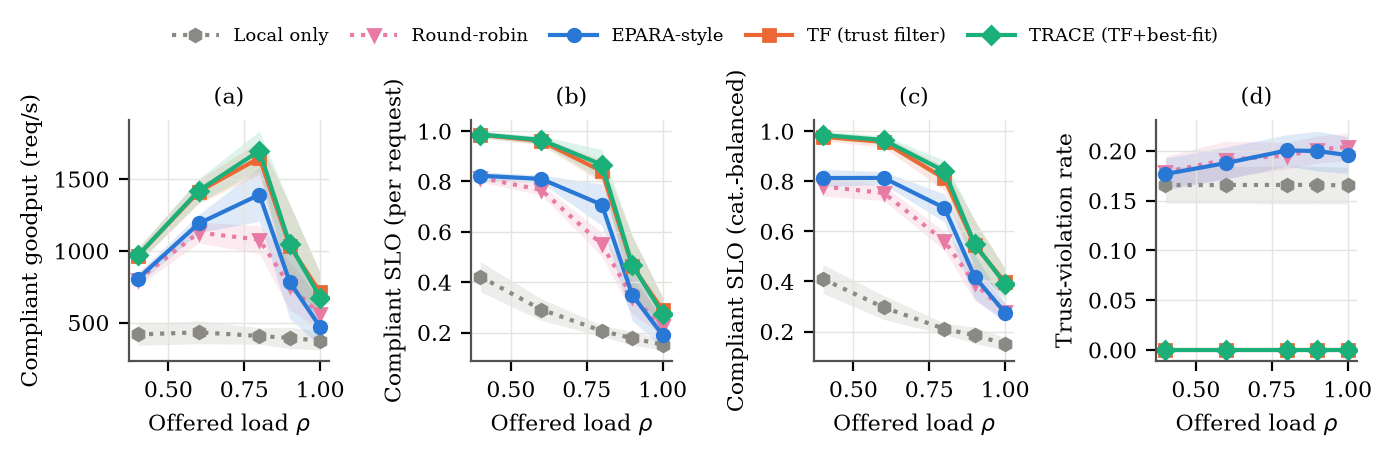
\includegraphics[width=\textwidth]{figures/fig_load.png}
\caption{Routing under increasing offered load (30 servers, 40\% sensitive traffic; mean and 95\% CI over 30 seeds). (a) Compliant SLO attainment and (b) its category-balanced version for compliant routers and references; (c) raw SLO attainment; (d) violation rate of trust-oblivious routers. Dashed lines are centralized oracles.}
\label{fig:2}
\end{figure*}

\begin{table*}[!t]
\centering
\caption{Routers at offered load \(\rho=0.8\) (mean ± 95\% CI over 30 seeds). SLO: raw SLO attainment; C-SLO: compliant SLO attainment, per request and category-balanced; Viol.: violation rate; C-goodput: compliant goodput (req/s); Fwd.: forwards per request; Shed: share of requests shed; µs/dec.: routing time per decision in the Python prototype.}
\footnotesize
\begin{adjustbox}{max width=\textwidth}
\begin{tabular}{lllllllll}
\toprule
Policy & SLO & C-SLO & C-SLO\_bal & Viol. & C-goodput & Fwd. & Shed & µs/dec. \\
\midrule
Local only & 0.574±0.015 & 0.466±0.013 & 0.450±0.011 & 0.107±0.007 & 907±31 & 0.00 & 0.426 & 0.0 \\
Round-robin & 0.931±0.005 & 0.743±0.009 & 0.694±0.008 & 0.188±0.007 & 1445±37 & 0.76 & 0.069 & 2.8 \\
EPARA-style & 0.986±0.001 & 0.788±0.007 & 0.744±0.011 & 0.199±0.007 & 1533±40 & 0.60 & 0.014 & 16.4 \\
Central oracle (no trust) & 1.000±0.000 & 0.802±0.008 & 0.788±0.009 & 0.197±0.008 & 1562±42 & 0.43 & 0.000 & 0.0 \\
TF-RR & 0.870±0.009 & 0.870±0.009 & 0.825±0.010 & 0.000±0.000 & 1694±43 & 0.88 & 0.130 & 3.5 \\
TF-P2C & 0.929±0.009 & 0.929±0.009 & 0.890±0.009 & 0.000±0.000 & 1808±46 & 0.78 & 0.071 & 16.6 \\
TF-JSQ & 0.956±0.007 & 0.956±0.007 & 0.918±0.007 & 0.000±0.000 & 1861±47 & 0.68 & 0.044 & 9.3 \\
Static pools & 0.673±0.039 & 0.673±0.039 & 0.704±0.032 & 0.000±0.000 & 1311±82 & 1.02 & 0.327 & 14.4 \\
TF & 0.950±0.007 & 0.950±0.007 & 0.899±0.009 & 0.000±0.000 & 1848±46 & 0.65 & 0.050 & 16.0 \\
TRACE & 0.960±0.006 & 0.960±0.006 & 0.908±0.009 & 0.000±0.000 & 1868±47 & 0.63 & 0.040 & 18.3 \\
Central oracle (trust) & 0.988±0.005 & 0.988±0.005 & 0.980±0.006 & 0.000±0.000 & 1924±51 & 0.83 & 0.012 & 0.0 \\
RR, shared pointer & 0.933±0.006 & 0.744±0.008 & 0.694±0.008 & 0.190±0.007 & 1447±35 & 0.77 & 0.067 & 2.5 \\
\bottomrule
\end{tabular}
\end{adjustbox}
\end{table*}

\subsection{Share of sensitive traffic and adaptive best-fit clearance}

Fig. 3 varies the share of sensitive requests from 0 to 80\%. The cost of compliance grows with the sensitive share because the set of eligible servers shrinks: the compliant oracle falls from 0.998 to 0.896, and the gap to the unconstrained oracle grows from 0.2 to 10.4 points. TRACE follows the same trend from 0.986 to 0.854 and stays 1.2 to 4.5 points below the compliant oracle.

Best-fit clearance helps exactly where the analysis of Section IV-B predicts. Its gain over TF is zero at 0\% and 20\% sensitive traffic and grows to +1.0, +2.2 and +2.4 points at 40\%, 60\% and 80\% (all \(p_H<2\times10^{-6}\)), and the category-balanced gains are similar (+0.9 to +1.9 points). When best-fit is always on, it costs 1.3 points with no sensitive traffic (\(p_H=2\times10^{-8}\)). The adaptive rule removes this cost: TRACE is indistinguishable from TF at 0\% and 20\% (\(p_H=1\)) and identical to always-on best-fit from 40\% upward. The parameters of the rule were fixed beforehand on separate tuning seeds (Table IV): \(\gamma=0.3\) had the largest mean gain across sensitive shares, and the gain changed sign between 20\% and 40\%, which gave the threshold \(q^\ast=30\%\). These evaluation results, on different seeds, confirm the choice.

Static pools behave in the opposite way. With little sensitive traffic, most requests compete for the few clearance-0 servers, and static pools collapse (0.156 at 0\%, 0.409 at 20\%). When most traffic is sensitive, the pools match the traffic and static partitioning becomes competitive: at 60\% and 80\% sensitive traffic it is statistically tied with TRACE (\(\Delta=+0.032\), \(p_H=1\), and \(\Delta=-0.017\), \(p_H=0.19\)). Adaptive routing is therefore most valuable when the sensitive share is unknown or changes over time.

\begin{figure*}[!t]
\centering
\includegraphics[width=\textwidth]{figures/fig_sens.png}
\caption{Effect of the share of sensitive requests (\(\rho=0.8\), 30 seeds). (a) Raw and (b) compliant SLO attainment; (c) paired gain of adaptive best-fit (TRACE) and of always-on best-fit over the plain trust filter.}
\label{fig:3}
\end{figure*}

\begin{table*}[!t]
\centering
\caption{Tuning of best-fit strength \(\gamma\) on the separate tuning seeds (1001--1010): mean paired gain in C-SLO over \(\gamma=1\) (plain TF) for each share of sensitive traffic (\(\rho=0.8\)).}
\footnotesize
\begin{adjustbox}{max width=\textwidth}
\begin{tabular}{lllllll}
\toprule
γ & 0\% & 20\% & 40\% & 60\% & 80\% & mean \\
\midrule
0.5 & -0.004 & +0.005 & +0.008 & +0.016 & +0.007 & +0.0062 \\
0.3 & -0.012 & -0.000 & +0.012 & +0.018 & +0.016 & +0.0066 \\
0.1 & -0.045 & -0.016 & +0.010 & +0.025 & +0.027 & +0.0001 \\
\bottomrule
\end{tabular}
\end{adjustbox}
\end{table*}

\subsection{When sensitive data originates at high-clearance sites}

The violation rate of a trust-oblivious router is set by the label distributions (Section III-E). Fig. 4 tests how much of it remains when sensitive data originates where it may be processed. With full alignment (\(\lambda=1\)), local-only service causes no violations, as Eq. (4) predicts, but offloading still does: the EPARA-style router violates for 13.5\% of requests and the unconstrained oracle for 9.9\%, because a sensitive request that cannot be served at its ingress server is offloaded to whichever peer has capacity, eligible or not. The violation rate therefore falls only from 19.9\% to 13.5\% for the EPARA-style router. Alignment barely changes the compliant routers (TRACE 0.960, 0.960 and 0.958 at \(\lambda=0\), 0.5 and 1), nor the cost of compliance under perfect information (1.2, 0.8 and 0.8 points). In short, aligning data with clearance makes violations rarer but does not remove the need for a trust filter in the router.

\begin{figure}[!t]
\centering
\includegraphics[width=\columnwidth]{figures/fig_corr.png}
\caption{Alignment between data sensitivity and ingress clearance (\(\lambda\) is the share of requests that originate at a server whose clearance covers them; \(\rho=0.8\), 30 seeds). (a) Violation rate of trust-oblivious routing; (b) compliant SLO attainment.}
\label{fig:4}
\end{figure}

\subsection{Overload and SLO-aware admission}

Table V isolates the admission rule. When every router processes requests that can no longer meet their SLO (``serve late''), all of them collapse at saturation: C-SLO at \(\rho=1.0\) is between 0.07 and 0.25 and the compliant oracle reaches only 0.20. Late work occupies slots without contributing goodput and delays everything queued behind it, so the backlog grows without bound. Shedding requests that can no longer meet their SLO lifts every router, by 51 to 76 points at \(\rho=1.0\) and by 50 to 70 points at \(\rho=1.2\) (all \(p_H<4\times10^{-8}\)). The admission rule, not the choice of peer, is the decisive design element in overload, and it is simple to add to any of the routers.

We also tested two fallbacks for the moment when the local view shows no eligible peer with spare capacity. Probing an eligible peer uniformly at random is neutral (within ±1.1 points of TF with either admission rule, \(p_H\ge0.25\)). A power-of-two-choices probe on synchronized backlog is harmful, by 1.1 to 5.9 points (\(p_H\le5\times10^{-4}\)), because it adds forwards toward peers that are themselves saturated. With shedding in place, no fallback is needed.

\begin{table}[!t]
\centering
\caption{Compliant SLO attainment in overload with and without SLO-aware admission (30 seeds). ``Serve late'' executes requests that can no longer meet their SLO; ``shed'' rejects them.}
\footnotesize
\begin{adjustbox}{max width=\columnwidth}
\begin{tabular}{lllll}
\toprule
Policy & ρ=1.0 serve late & ρ=1.0 shed & ρ=1.2 serve late & ρ=1.2 shed \\
\midrule
EPARA-style & 0.067±0.015 & 0.728±0.010 & 0.016±0.002 & 0.545±0.025 \\
TF-RR & 0.245±0.017 & 0.752±0.013 & 0.119±0.011 & 0.633±0.016 \\
TF-P2C & 0.137±0.027 & 0.814±0.014 & 0.020±0.005 & 0.651±0.019 \\
TF & 0.158±0.042 & 0.875±0.010 & 0.034±0.007 & 0.719±0.022 \\
TF + uniform probe & 0.162±0.029 & 0.875±0.009 & 0.029±0.005 & 0.730±0.022 \\
TF + P2C fallback & 0.099±0.032 & 0.864±0.009 & 0.008±0.004 & 0.678±0.024 \\
TRACE & 0.136±0.032 & 0.895±0.010 & 0.031±0.005 & 0.733±0.024 \\
Central oracle (trust) & 0.203±0.088 & 0.859±0.020 & 0.007±0.006 & 0.503±0.033 \\
\bottomrule
\end{tabular}
\end{adjustbox}
\end{table}

\subsection{State staleness}

Fig. 5 varies the synchronization period \(H\). With SLO-aware admission, fresher state helps the capacity-proportional routers at both loads: TRACE gains 2.5 points at \(\rho=0.8\) and 5.0 points at \(\rho=1.0\) when \(H\) falls from 2 s to 0.1 s (\(p_H<10^{-4}\)), and TF behaves alike. TF-JSQ, which acts deterministically on the synchronized backlog, benefits least from fresh state at \(\rho=1.0\) (+1.4 points, \(p_H=0.15\)), and it is 3.3 to 8.1 points behind TRACE at that load for every \(H\) tested. At \(\rho=0.8\), TRACE and TF-JSQ are tied for both short and long sync periods.

\begin{figure}[!t]
\centering
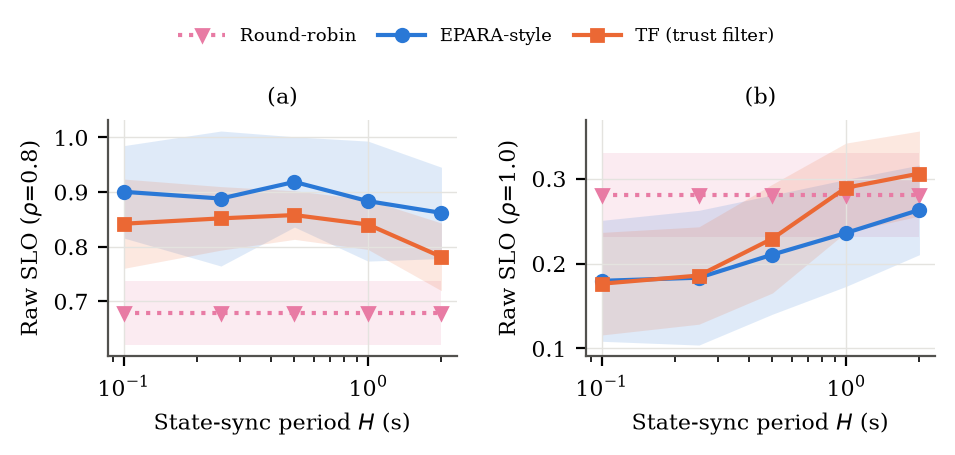
\includegraphics[width=\columnwidth]{figures/fig_stale.png}
\caption{Sensitivity to the state-sync period \(H\) at (a) \(\rho=0.8\) and (b) \(\rho=1.0\) (20 seeds).}
\label{fig:5}
\end{figure}

\subsection{Partial placement and a cloud fallback}

Table VI relaxes two simplifications. When each service is hosted on only half of the servers (at least one per domain), all routers lose: TRACE falls from 0.961 to 0.906, because fewer eligible servers host each service. A cloud tier with 96 slots, 40 ms one-way latency and clearance 1 recovers part of this loss (TRACE 0.932 with partial placement and 0.970 with full placement), while serving only 0.9\% to 2.7\% of the requests. The cloud cannot help sensitivity-2 requests, which must stay in their domain. TRACE's advantage over the EPARA-style router is stable across all four settings (+14.1 to +16.9 points, \(p_H<10^{-5}\)).

\begin{table*}[!t]
\centering
\caption{Partial placement and a cloud fallback (\(\rho=0.8\), 20 seeds). Placement: share of servers hosting each service.}
\footnotesize
\begin{adjustbox}{max width=\textwidth}
\begin{tabular}{lllllll}
\toprule
Placement & Cloud & EPARA-style C-SLO & TF C-SLO & TRACE C-SLO & TRACE cloud share & EPARA viol. \\
\midrule
100\% & no & 0.792±0.008 & 0.951±0.008 & 0.961±0.007 & 0.000 & 0.195 \\
100\% & yes & 0.803±0.008 & 0.962±0.007 & 0.970±0.007 & 0.009 & 0.197 \\
50\% & no & 0.748±0.021 & 0.896±0.019 & 0.906±0.017 & 0.000 & 0.200 \\
50\% & yes & 0.791±0.016 & 0.921±0.015 & 0.932±0.015 & 0.027 & 0.208 \\
\bottomrule
\end{tabular}
\end{adjustbox}
\end{table*}

\subsection{Robustness to parameters and topology}

Appendix Table IX varies one parameter at a time (10 seeds). TRACE stays within 0.919 and 0.981 C-SLO in every setting and is ahead of TF in every one. The largest effects are structural: allowing only one forward (\(K_{\max}=1\)) costs 4.3 points, and more trust domains cost capacity for sensitivity-2 requests (0.981 with one domain, 0.942 with five). A short capacity horizon (\(\Delta=0.1\) s) costs 1.9 points; the proximity scale \(\ell_0\) has no measurable effect, and removing the fit preference (factor 0) slightly helps. With fewer high-clearance servers (clearance mix 0.5/0.3/0.2), TRACE falls to 0.933, and with more (0.2/0.4/0.4) it rises to 0.972.

Confidence intervals across seeds are dominated by topology. Running five arrival sequences on each of ten topologies, the topology accounts for 88\% of the variance of the EPARA-style router's C-SLO and 58\% of TRACE's (intraclass correlation). TRACE's gain over the EPARA-style router, however, is positive on every topology (+12.6 to +18.5 points), and it is not correlated with the share of capacity eligible for sensitivity-2 requests (Spearman \(-0.04\), \(p=0.91\)). Paired comparisons over seeds, which cancel the topology effect, are therefore the appropriate test, and they are what we report.

\subsection{Scale and decision overhead}

Fig. 6 varies the number of servers from 10 to 120 (10 seeds). TRACE's C-SLO rises with scale (0.894 at \(N=10\), 0.979 at \(N=120\)), because larger systems contain more eligible peers at every sensitivity level, and it is at or above TF, TF-P2C and TF-RR at every size. A routing decision takes 17 to 20 µs in our Python prototype (measured while two simulations shared two CPU cores), almost independent of \(N\) because the per-peer arithmetic is vectorized; TF-RR is cheaper (3 µs) but routes worse. This is nearly four orders of magnitude below the tightest SLO of 150 ms, and the decision needs no communication. The cost that does grow with \(N\) is the age of the synchronized view (Section IV-C), which our simulator does not model and which we leave to future work.

\begin{figure}[!t]
\centering
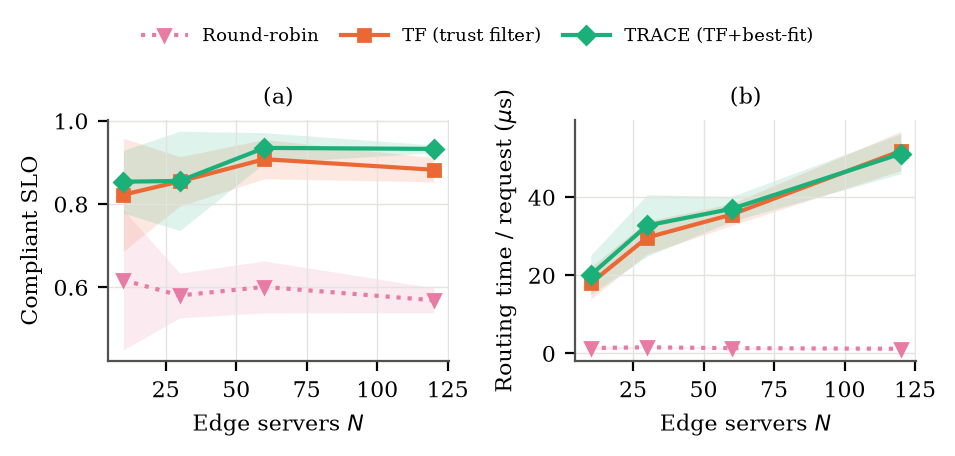
\includegraphics[width=\columnwidth]{figures/fig_scale.png}
\caption{Scaling the number of edge servers (\(\rho=0.8\), 10 seeds): (a) compliant SLO attainment, (b) routing time per decision.}
\label{fig:6}
\end{figure}

\section{Energy-Aware Routing: A Hypothesis Test}

\textbf{Hypothesis.} On power-capped, solar or battery-backed sites, scaling the offload score by peers' energy headroom should raise compliant SLO attainment, because it steers work away from servers that are about to throttle or go offline. We test this hypothesis with the five variants of Section IV-D on top of TF, under both energy models, with constant supply at \(\Phi\in\{0.6,0.9,1.2\}\) and with phase-shifted solar supply at \(\Phi\in\{0.9,1.2\}\), in 180 s runs measured after a 60 s warm-up from a random initial charge (10 seeds; Tables VII and VIII, Fig. 7). For each experiment, the 30 (constant supply) or 20 (solar) comparisons with TF form one Holm family.

\textbf{Energy scarcity with soft throttling.} When supply is well below demand (\(\Phi=0.6\)), steering by energy hurts. TF+EW loses 9.2 points and TF+EC 15.8 points against TF (0.934), while the bounded variant that only deprioritizes is indistinguishable from TF (+0.0 points). The losses are consistent across seeds (TF+EW and TF+EC lose on every seed) but, with 10 seeds and 30 tests in the family, their Holm-adjusted \(p\)-values are 0.06 and 0.06. The mechanism is visible in the measured dispersion: TF+EW raises the coefficient of variation of per-server utilization from 0.20 to 0.26 and forwards per request from 0.70 to 0.97, and TF+EC raises the utilization CV to 0.30. Work is concentrated on the servers that currently hold energy, while servers with low headroom but idle slots, which could still run short jobs, are avoided. Energy weighting does reduce throttling (throttled fraction 37.2\% instead of 51.1\%), but the extra forwarding and concentration cost more SLO attainment than the avoided throttling saves. Even perfect energy information does not help here: the feasibility oracle TF+EF loses 3.4 points, because excluding servers that cannot finish a job without throttling also excludes capacity that would have served the job within its SLO.

\textbf{Hard outages.} Under the outage model the penalty disappears. TF+EW is level with TF when energy is scarce (+0.1 points at \(\Phi=0.6\)) and slightly ahead when supply is closer to demand (+0.8 and +0.7 points at \(\Phi=0.9\) and 1.2, ahead on 9 of 10 seeds), and it keeps more servers online: at \(\Phi=0.9\), availability rises from 0.888 to 0.957 and drain events fall from 6.3 to 2.5 per minute. Avoiding peers that are close to their outage threshold prevents the outage itself, which removes a whole server's capacity for the recharge period. The gains are small, however, and none is significant after correction (smallest Holm-adjusted \(p\): 0.09). TF+EC coincides with TF under this model, because its energy capacity binds only when a buffer is nearly empty or overdrawn, and such servers are already offline.

\textbf{Sufficient and heterogeneous supply.} When aggregate supply exceeds demand (\(\Phi=1.2\)), with constant or phase-shifted solar supply, every variant is within 0.7 points of TF, and no difference is significant. With solar supply at \(\Phi=0.9\), so that some sites are in surplus while others are in deficit, the picture is the same as with constant supply but weaker: TF+EW loses 0.7 points under soft throttling and gains +1.4 points under outage, neither significant after correction. Shifting work toward sites that currently have surplus energy, which is the scenario in which energy-aware routing seemed most promising, therefore yields no measurable benefit at the per-request timescale in our setting.

\textbf{Timescales and staleness.} With a short 20 s buffer the soft-throttling penalty of TF+EW remains (−8.7 points) and the outage gain is +1.4 points; with a 600 s buffer, all variants coincide with TF (within 0.1 points). Under solar supply at \(\Phi=0.9\) with outages, the difference between TF+EW and TF is +1.1 points with fresh state (\(H=0.1\) s) and +0.8 points with stale state (\(H=2\) s), so staleness does not change the conclusion.

\textbf{Conclusion of the test.} The hypothesis is not supported as a general rule. Energy-headroom weighting is harmful when energy is scarce and an empty buffer slows work down, gives small and statistically unconfirmed gains when an empty buffer takes a server offline, and is neutral when supply is sufficient. A bounded weight that never excludes a peer is harmless in every regime but also never helps significantly. At the per-request timescale, energy information is best used as a feasibility check at the processing server and, if hard outages are expected, as a mild preference against peers near their outage threshold; larger gains, if any, are more likely at slower layers that can act on forecasts, such as service placement, admission control and DVFS.

\begin{figure*}[!t]
\centering
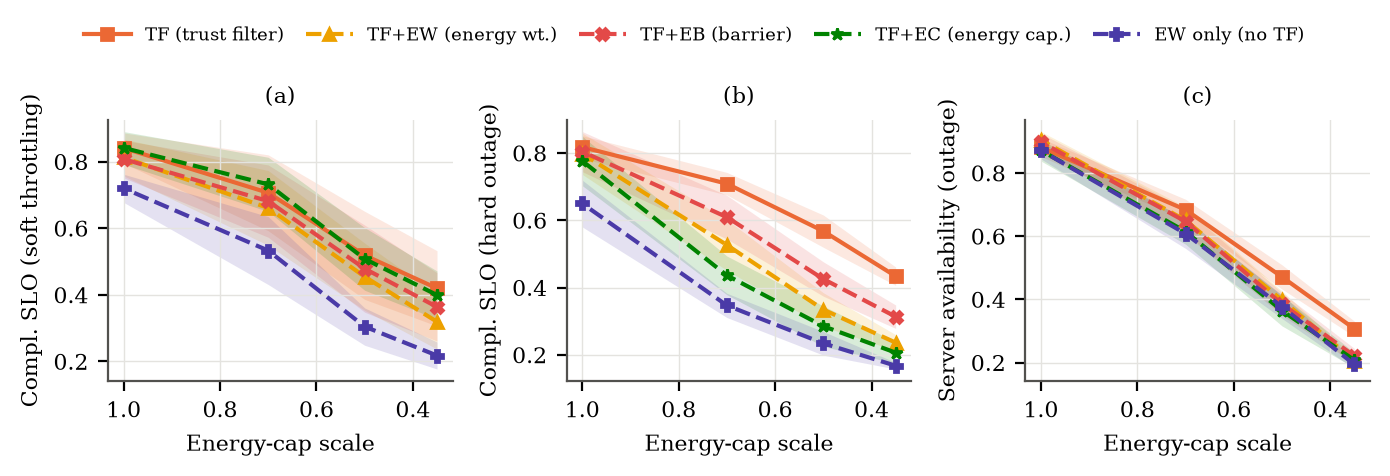
\includegraphics[width=\textwidth]{figures/fig_energy.png}
\caption{Energy-aware variants as the supply ratio \(\Phi\) varies (constant supply, \(\rho=0.8\), 10 seeds). Compliant SLO attainment under (a) soft throttling and (b) hard outages; (c) coefficient of variation of per-server utilization and (d) mean server availability under hard outages.}
\label{fig:7}
\end{figure*}

\begin{table*}[!t]
\centering
\caption{Compliant SLO attainment of energy-aware variants with constant supply (180 s runs, 10 seeds).}
\footnotesize
\begin{adjustbox}{max width=\textwidth}
\begin{tabular}{llllllll}
\toprule
Φ & Model & TF & TF+EW & TF+EB & TF+EC & TF+EW-bounded & TF+EF (oracle feas.) \\
\midrule
0.6 & soft & 0.93±0.01 & 0.84±0.02 & 0.91±0.01 & 0.78±0.02 & 0.93±0.01 & 0.90±0.02 \\
0.6 & outage & 0.66±0.03 & 0.66±0.04 & 0.66±0.03 & 0.66±0.03 & 0.66±0.03 & 0.64±0.03 \\
0.9 & soft & 0.93±0.01 & 0.93±0.01 & 0.94±0.01 & 0.92±0.01 & 0.94±0.01 & 0.94±0.01 \\
0.9 & outage & 0.91±0.01 & 0.92±0.01 & 0.91±0.01 & 0.91±0.01 & 0.91±0.01 & 0.90±0.01 \\
1.2 & soft & 0.94±0.01 & 0.94±0.00 & 0.94±0.01 & 0.94±0.01 & 0.94±0.00 & 0.94±0.01 \\
1.2 & outage & 0.94±0.00 & 0.94±0.00 & 0.94±0.01 & 0.94±0.00 & 0.94±0.01 & 0.94±0.00 \\
\bottomrule
\end{tabular}
\end{adjustbox}
\end{table*}

\begin{table*}[!t]
\centering
\caption{Compliant SLO attainment with phase-shifted solar supply (three time zones; 10 seeds).}
\footnotesize
\begin{adjustbox}{max width=\textwidth}
\begin{tabular}{llllllll}
\toprule
Φ & Model & TF & TF+EW & TF+EB & TF+EC & TF+EW-bounded & TF+EF (oracle feas.) \\
\midrule
0.9 & soft & 0.93±0.01 & 0.93±0.01 & 0.94±0.01 & 0.92±0.01 & 0.94±0.01 & 0.92±0.01 \\
0.9 & outage & 0.90±0.02 & 0.91±0.01 & 0.91±0.01 & 0.90±0.02 & 0.91±0.02 & 0.90±0.02 \\
1.2 & soft & 0.94±0.01 & 0.94±0.00 & 0.95±0.01 & 0.94±0.01 & 0.94±0.01 & 0.94±0.01 \\
1.2 & outage & 0.94±0.00 & 0.94±0.00 & 0.94±0.01 & 0.94±0.00 & 0.94±0.01 & 0.94±0.01 \\
\bottomrule
\end{tabular}
\end{adjustbox}
\end{table*}

\section{Discussion}

\textbf{What the results say about compliant routing.} Three design elements matter, in decreasing order of effect. First, SLO-aware admission decides whether a router survives saturation at all: without it, every router we evaluated, including a centralized oracle, served fewer than a quarter of requests on time at \(\rho=1.0\). Second, the trust filter is a precondition, not an optimization: a router that ignores the constraint violates it for a share of requests that is fixed by the label distributions, and aligning data with clearance only reduces that share. Third, among compliant routers the choice of peer matters most near saturation, where capacity-proportional sampling outperforms round-robin, power-of-two choices and join-the-shortest-queue; below saturation, TF-JSQ is equally good. Best-fit clearance is a modest refinement worth about one to two points when a substantial share of traffic is sensitive, and the adaptive rule makes it safe to leave enabled. We therefore regard the trust filter with SLO-aware admission as the core of TRACE and best-fit clearance as an optional component.

\textbf{Cost of compliance.} With perfect information, compliance costs 1.2 points of SLO attainment at the default sensitive share and up to 10 points when 80\% of the traffic is sensitive; at the default share, a decentralized router pays about twice as much (2.7 points). The cost is driven by the capacity that is eligible for the most restrictive class, so it is a property of the deployment (how many servers carry which clearance in which domain) as much as of the router. Trust-aware service placement, which we hold fixed, is the natural lever to reduce it further.

\textbf{Static partitioning.} Dedicated pools per sensitivity tier are simple to audit, and they match TRACE when the pools are sized to the traffic, as they happen to be in our setting at 60--80\% sensitive traffic. They fail badly when the traffic mix and the pool sizes diverge (0.16 to 0.67 C-SLO at 0--40\% sensitive traffic). Routing that lets less sensitive requests use idle higher-clearance capacity removes this sizing problem.

\textbf{Implications for EPARA-style systems.} The trust filter is a small, local change to EPARA's handler: a per-peer eligibility test on static, attested labels, with decisions in tens of microseconds and no extra communication. SLO-aware admission is a local check as well. Because the violation rate of a trust-oblivious handler is set by the deployment rather than by the router, we argue that edge inference systems that handle regulated data should report goodput subject to compliance, together with the cost of compliance against a reference, rather than raw goodput alone.

\textbf{Energy awareness.} Energy-headroom weighting did not hold up as a general improvement (Section VII). Every policy draws on the same energy income, so a router cannot create energy; it can only decide where work runs. When an empty buffer merely slows work down, avoiding low-headroom peers concentrates load and adds forwarding, which costs more than the throttling it prevents (9.2 points at \(\Phi=0.6\)). When an empty buffer takes a server offline, a mild preference against nearly drained peers prevents outages and slightly raises SLO attainment (+0.8 points at \(\Phi=0.9\), not significant after correction). Whether energy-aware routing helps therefore depends on how a site fails when energy runs out, which should be measured before such a policy is deployed.

\textbf{Threats to validity and limitations.} \emph{Simulation only.} All results come from an event-driven simulator. Service times, slot power, label distributions, energy supply and the network model are assumptions at the scale of EPARA's testbed, not measurements, and absolute values should not be compared with EPARA's results \cite{epara2025}. \emph{Operator abstraction.} EPARA's operators are reduced to fixed per-category slot and time profiles; batching gains, co-location interference and model loading are not modelled, so the evaluation concerns the request-handling layer only. \emph{Workload.} Arrivals are synthetic (Poisson with hot spots and bursts), not the Azure function and LLM traces used by EPARA \cite{epara2025,shahrad2020serverless}. \emph{Fixed layers.} Placement is either full replication or random partial replication; demand- and trust-aware placement is not evaluated. \emph{State dissemination.} Views are synchronized instantaneously every \(H\) seconds; the propagation delay of a ring, which grows with \(N\), and the bandwidth of synchronization are not modelled. \emph{Trust model.} Labels are static, attested and honest; eligibility follows a single rule (2), whereas real policies (consent, purpose limitation, cross-border transfer rules) are richer. \emph{References.} The centralized oracles are greedy earliest-finish dispatchers with perfect information, not proven optima; they are not upper bounds in overload. \emph{Energy model.} Energy is a buffer with fixed per-slot power; DVFS, idle power and cooling are not modelled, and solar supply is a compressed sinusoid rather than a measured profile. \emph{Statistics.} Trust experiments use 30 seeds (fewer for robustness and scale studies) and energy experiments 10 seeds; all claims rest on paired tests with Holm correction within declared families, and \(\gamma\) and \(q^\ast\) were tuned on separate seeds. \emph{Timing.} Decision times come from a Python prototype on a shared machine and are indicative only.

\section{Conclusion}

Decentralized, capacity-proportional request routing pools the scattered capacity of edge servers effectively, but routers designed this way treat every server as a lawful destination. We formulated trust-constrained routing for categorized edge inference as goodput maximization subject to zero violations, using multilevel-security labels and an explicit threat model, and showed that the violation rate of trust-oblivious routing is fixed by the label distributions. TRACE combines a hard trust filter, SLO-aware admission and an adaptive best-fit clearance preference with capacity-proportional offloading. Against trust-filtered round-robin, power-of-two-choices and join-the-shortest-queue routing, static pools and a centralized oracle, TRACE was the best or tied-best decentralized compliant router at every load (tied with join-the-shortest-queue below saturation), within about three points of the centralized oracle below saturation and ahead of it in overload; compliance cost 1.2 points with perfect information and 2.7 points for decentralized routing at the default sensitive share. SLO-aware admission was the single most important element, raising every router's SLO attainment at \(\rho=1.0\) by more than 50 points. Energy-headroom weighting, which we had expected to help on energy-constrained sites, did not hold up as a general rule: it lost 9.2 points when energy was scarce and an empty buffer throttled work, gained at most 1.4 points (not significant after correction) when an empty buffer caused an outage, and made no difference when supply was sufficient.

The next steps are to replace the assumed service and power profiles with measurements on edge hardware, to drive the simulator with production traces, to model state dissemination at scale, to co-design trust-aware service placement with the router, and to study energy awareness at the placement and admission-control layers, where forecasts can be used.

\section*{Data and Code Availability}

The simulator (ecsim.py), the experiment suite (experiments\_v3.py), the analysis script (analyze\_v3.py) and the raw per-run results (runs\_v3.jsonl, 6,040 runs) that produce every number, figure and table in this article are publicly available at https://github.com/gaurav3611/edge-cloud-ai-routing (branch revision-v3). The tuning seeds (1001--1010) and evaluation seeds are listed in the experiment script.

\section*{Acknowledgment}

This work received no external funding. The authors used Claude (Anthropic), an AI assistant, to help develop the simulation code, run and analyze the experiments, and draft and edit the manuscript; the authors reviewed and verified all content and take full responsibility for it.

\bibliographystyle{IEEEtran}
\bibliography{refs}

\appendices

\section{Parameter Sensitivity}

Table IX varies one routing or topology parameter at a time around the defaults of Table II (\(\rho=0.8\), 10 seeds). TRACE is ahead of TF in every setting.

\begin{table}[!t]
\centering
\caption{One-at-a-time sensitivity of compliant SLO attainment (\(\rho=0.8\), 10 seeds).}
\footnotesize
\begin{adjustbox}{max width=\columnwidth}
\begin{tabular}{llll}
\toprule
Parameter & Value & TF C-SLO & TRACE C-SLO \\
\midrule
(default) & Kmax=2, ℓ0=20 ms, Δ=0.5 s, 0.05, 3 dom., 0.3/0.4/0.3 & 0.951±0.008 & 0.962±0.007 \\
kmax & 1.0 & 0.903±0.011 & 0.919±0.011 \\
kmax & 3.0 & 0.959±0.007 & 0.968±0.008 \\
kmax & 4.0 & 0.961±0.006 & 0.969±0.007 \\
l0 & 0.005 & 0.951±0.007 & 0.962±0.007 \\
l0 & 0.08 & 0.949±0.006 & 0.961±0.006 \\
horizon & 0.1 & 0.930±0.007 & 0.943±0.009 \\
horizon & 0.25 & 0.945±0.007 & 0.956±0.006 \\
horizon & 1.0 & 0.947±0.008 & 0.962±0.006 \\
fitfac & 0.0 & 0.965±0.006 & 0.972±0.005 \\
fitfac & 0.2 & 0.949±0.006 & 0.962±0.007 \\
fitfac & 1.0 & 0.947±0.007 & 0.961±0.007 \\
n\_dom & 1.0 & 0.969±0.006 & 0.981±0.003 \\
n\_dom & 2.0 & 0.961±0.008 & 0.972±0.005 \\
n\_dom & 5.0 & 0.934±0.007 & 0.942±0.007 \\
clear\_p & (0.2, 0.4, 0.4) & 0.968±0.009 & 0.972±0.009 \\
clear\_p & (0.5, 0.3, 0.2) & 0.916±0.009 & 0.933±0.011 \\
\bottomrule
\end{tabular}
\end{adjustbox}
\end{table}

\section{Simulator Details}

The simulator processes arrivals in time order. Every \(H\) seconds it refreshes the view of every server: spare slots over the next \(\Delta\) seconds, computed by clipping each slot's remaining busy time to the horizon; the time until \(m\) slots become free, for \(m\in\{1,2,8\}\), used as the backlog estimate by TF-P2C and TF-JSQ; the online status; and, for the energy variants, the energy headroom \(E_j/B_j\). Between refreshes, a server debits its view of a peer by the work it has itself sent there, so different servers hold different views. A service occupying \(m\) slots starts when its \(m\) earliest-free slots are available. Energy is charged when a job is admitted, at \(P_s\) per slot for its duration, and the buffer refills continuously with the (constant or solar) supply. Network latency is added per forward. The centralized oracles evaluate every eligible, online server hosting the service with exact slot and energy state and the latency from the ingress server. Each seed fixes the topology, placement and arrival sequence, which are identical across routers, so comparisons are paired. A request is counted once, after the warm-up, as successful if it met its SLO, as a violation if it was processed at an ineligible server, and as shed if it was rejected.

\end{document}
